\appendix

\renewcommand{\thefigure}{A.\arabic{figure}}
\setcounter{figure}{0}

\addcontentsline{toc}{section}{Appendices}
\chapter*{ Appendix A: Screenshots}
\begin{figure}[H]
    \centering
    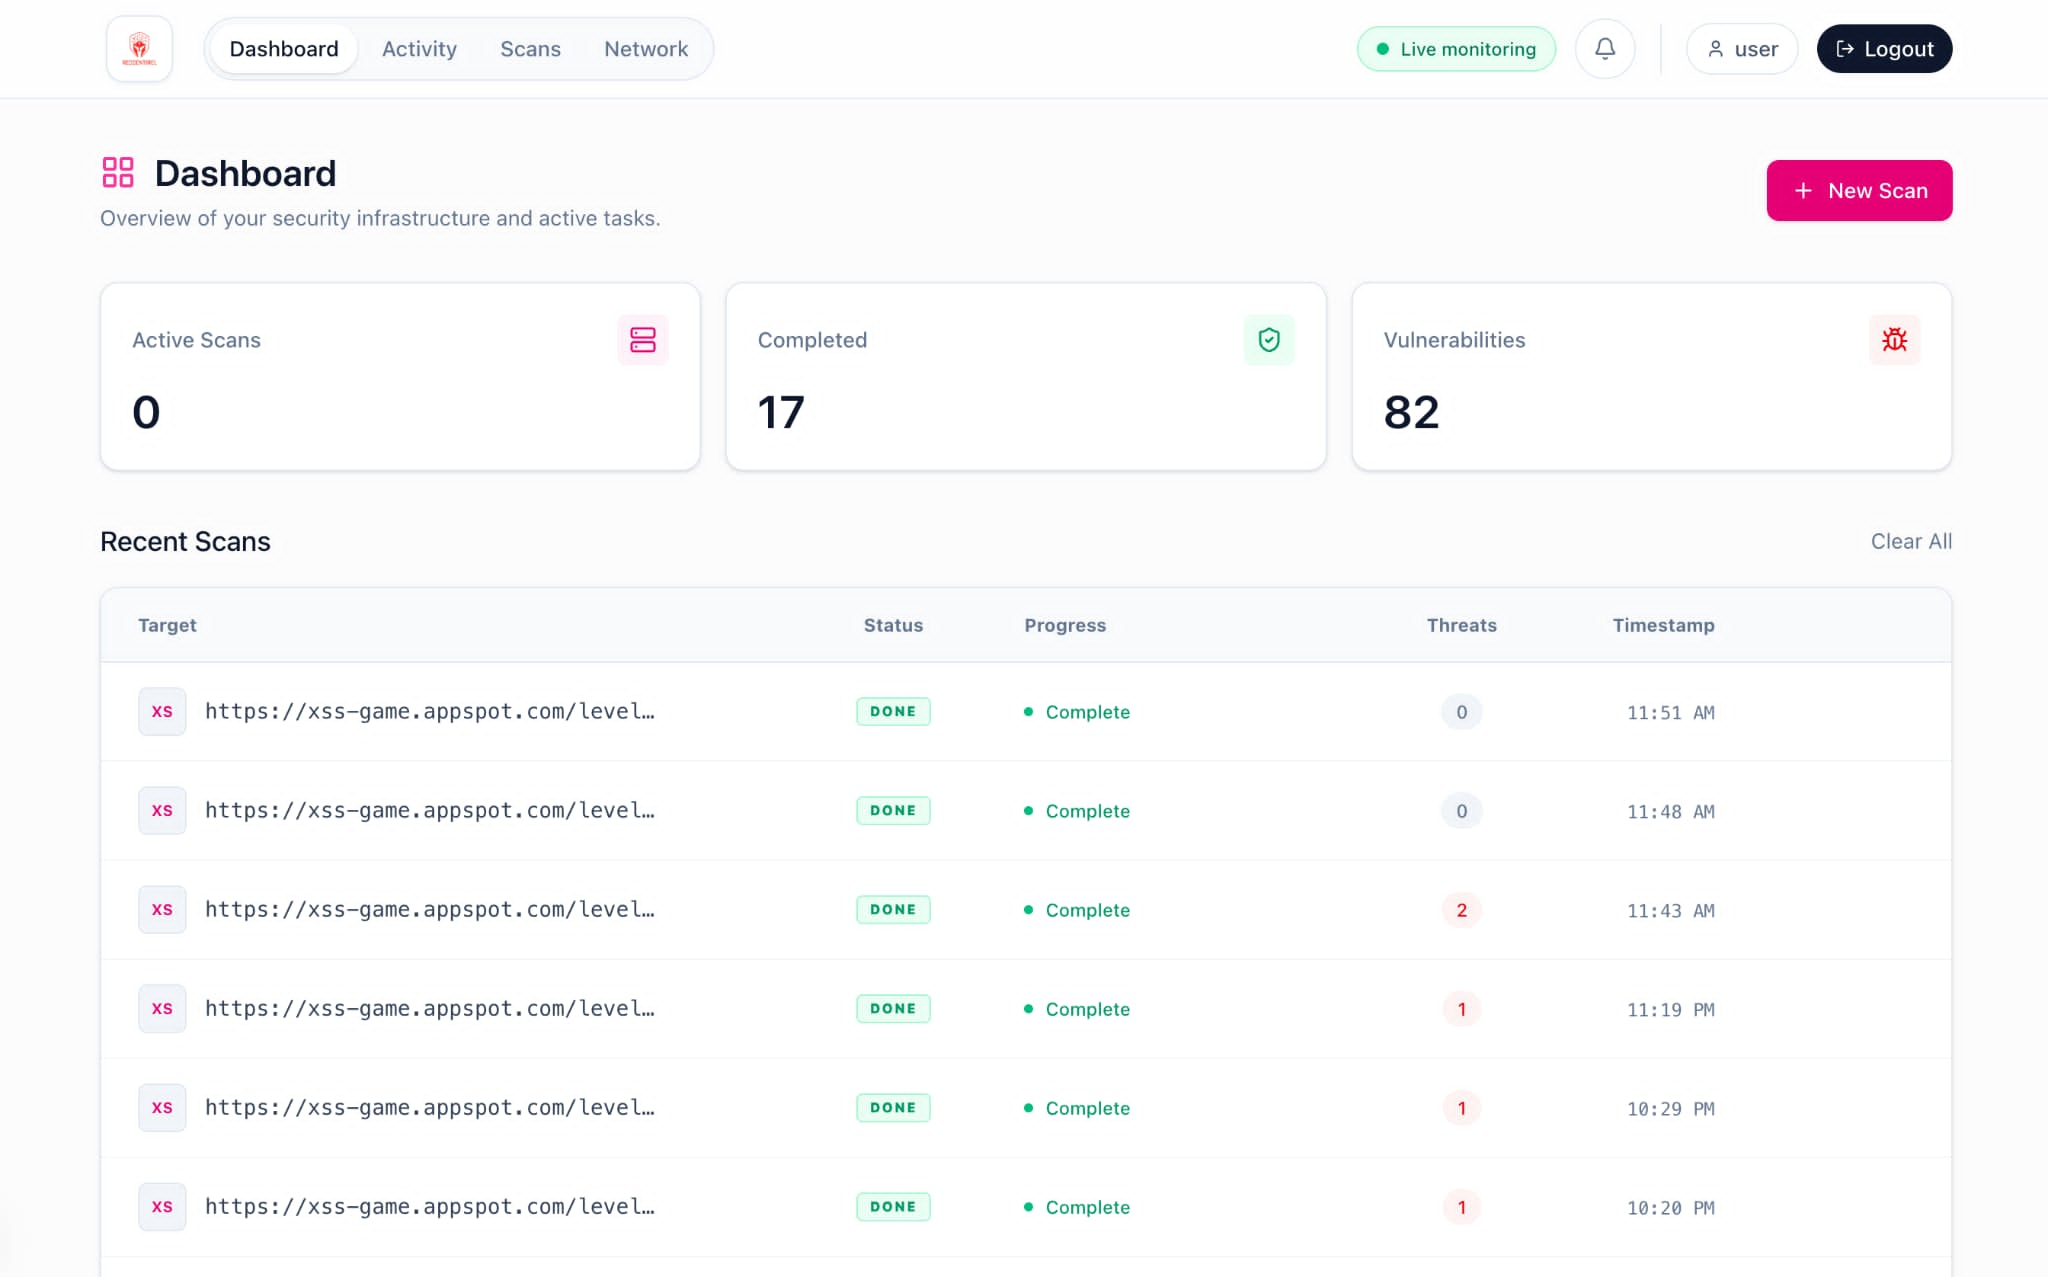
\includegraphics[width=1\linewidth]{figures/appendix/dashboard.jpg}
    \caption{RedSentinel Dashboard }
    \label{fig:appendix_new_scan}
\end{figure}
\begin{figure}[H]
    \centering
    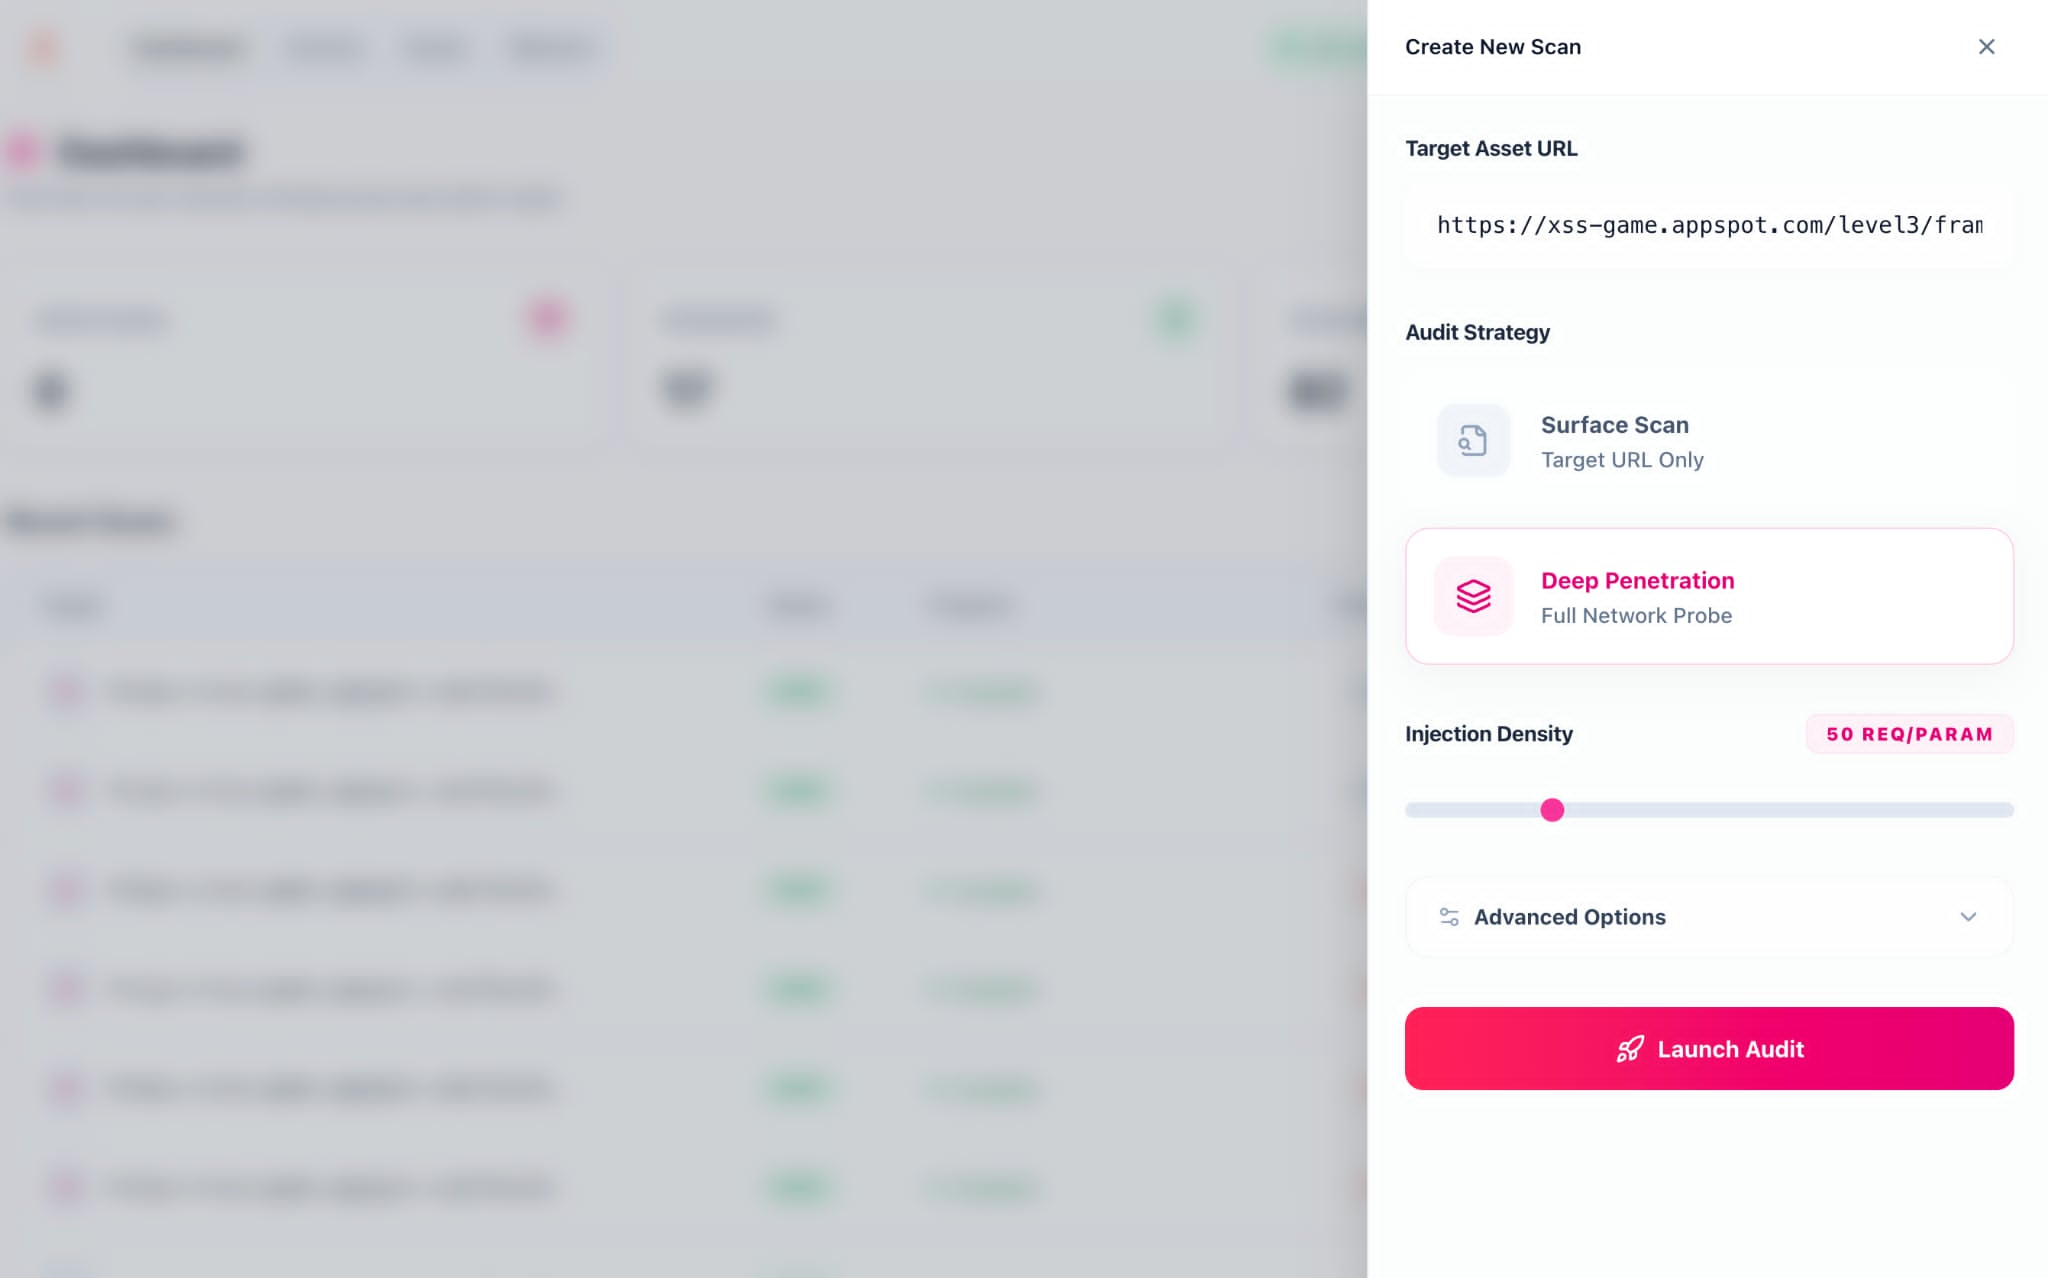
\includegraphics[width=1\textwidth]{figures/appendix/Scanmenu.jpg}
    \caption{New Scan Configuration}
    \label{fig:example_image}
\end{figure}
\begin{figure}[H]
    \centering
    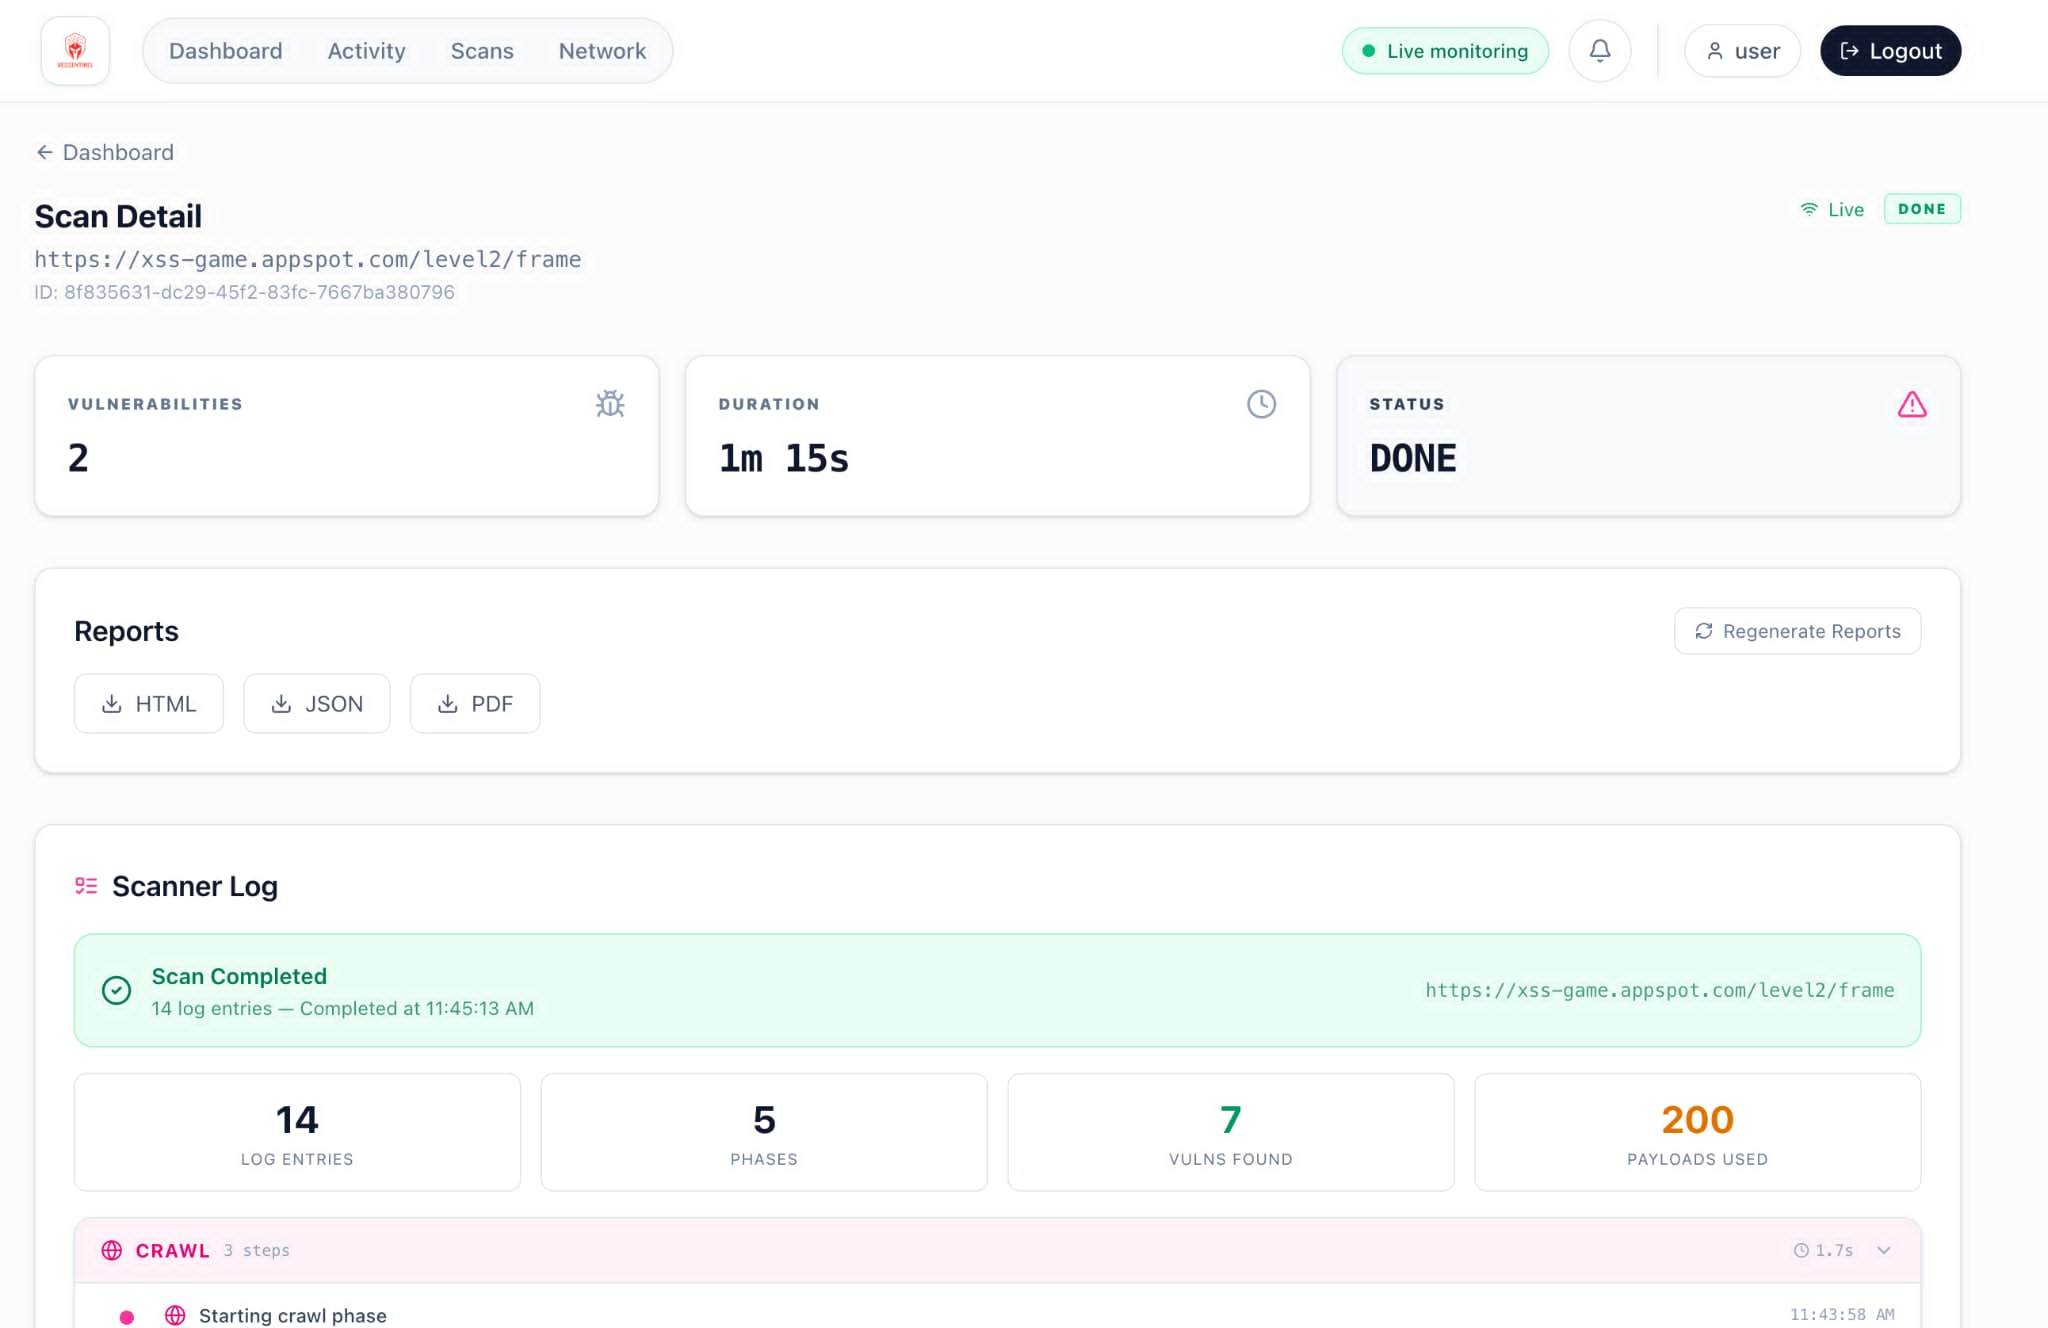
\includegraphics[width=1\textwidth]{figures/appendix/scandetail.jpg}
    \caption{Scan result}
    \label{fig:example_image}
    
\end{figure}
\begin{figure}[H]
    \centering
    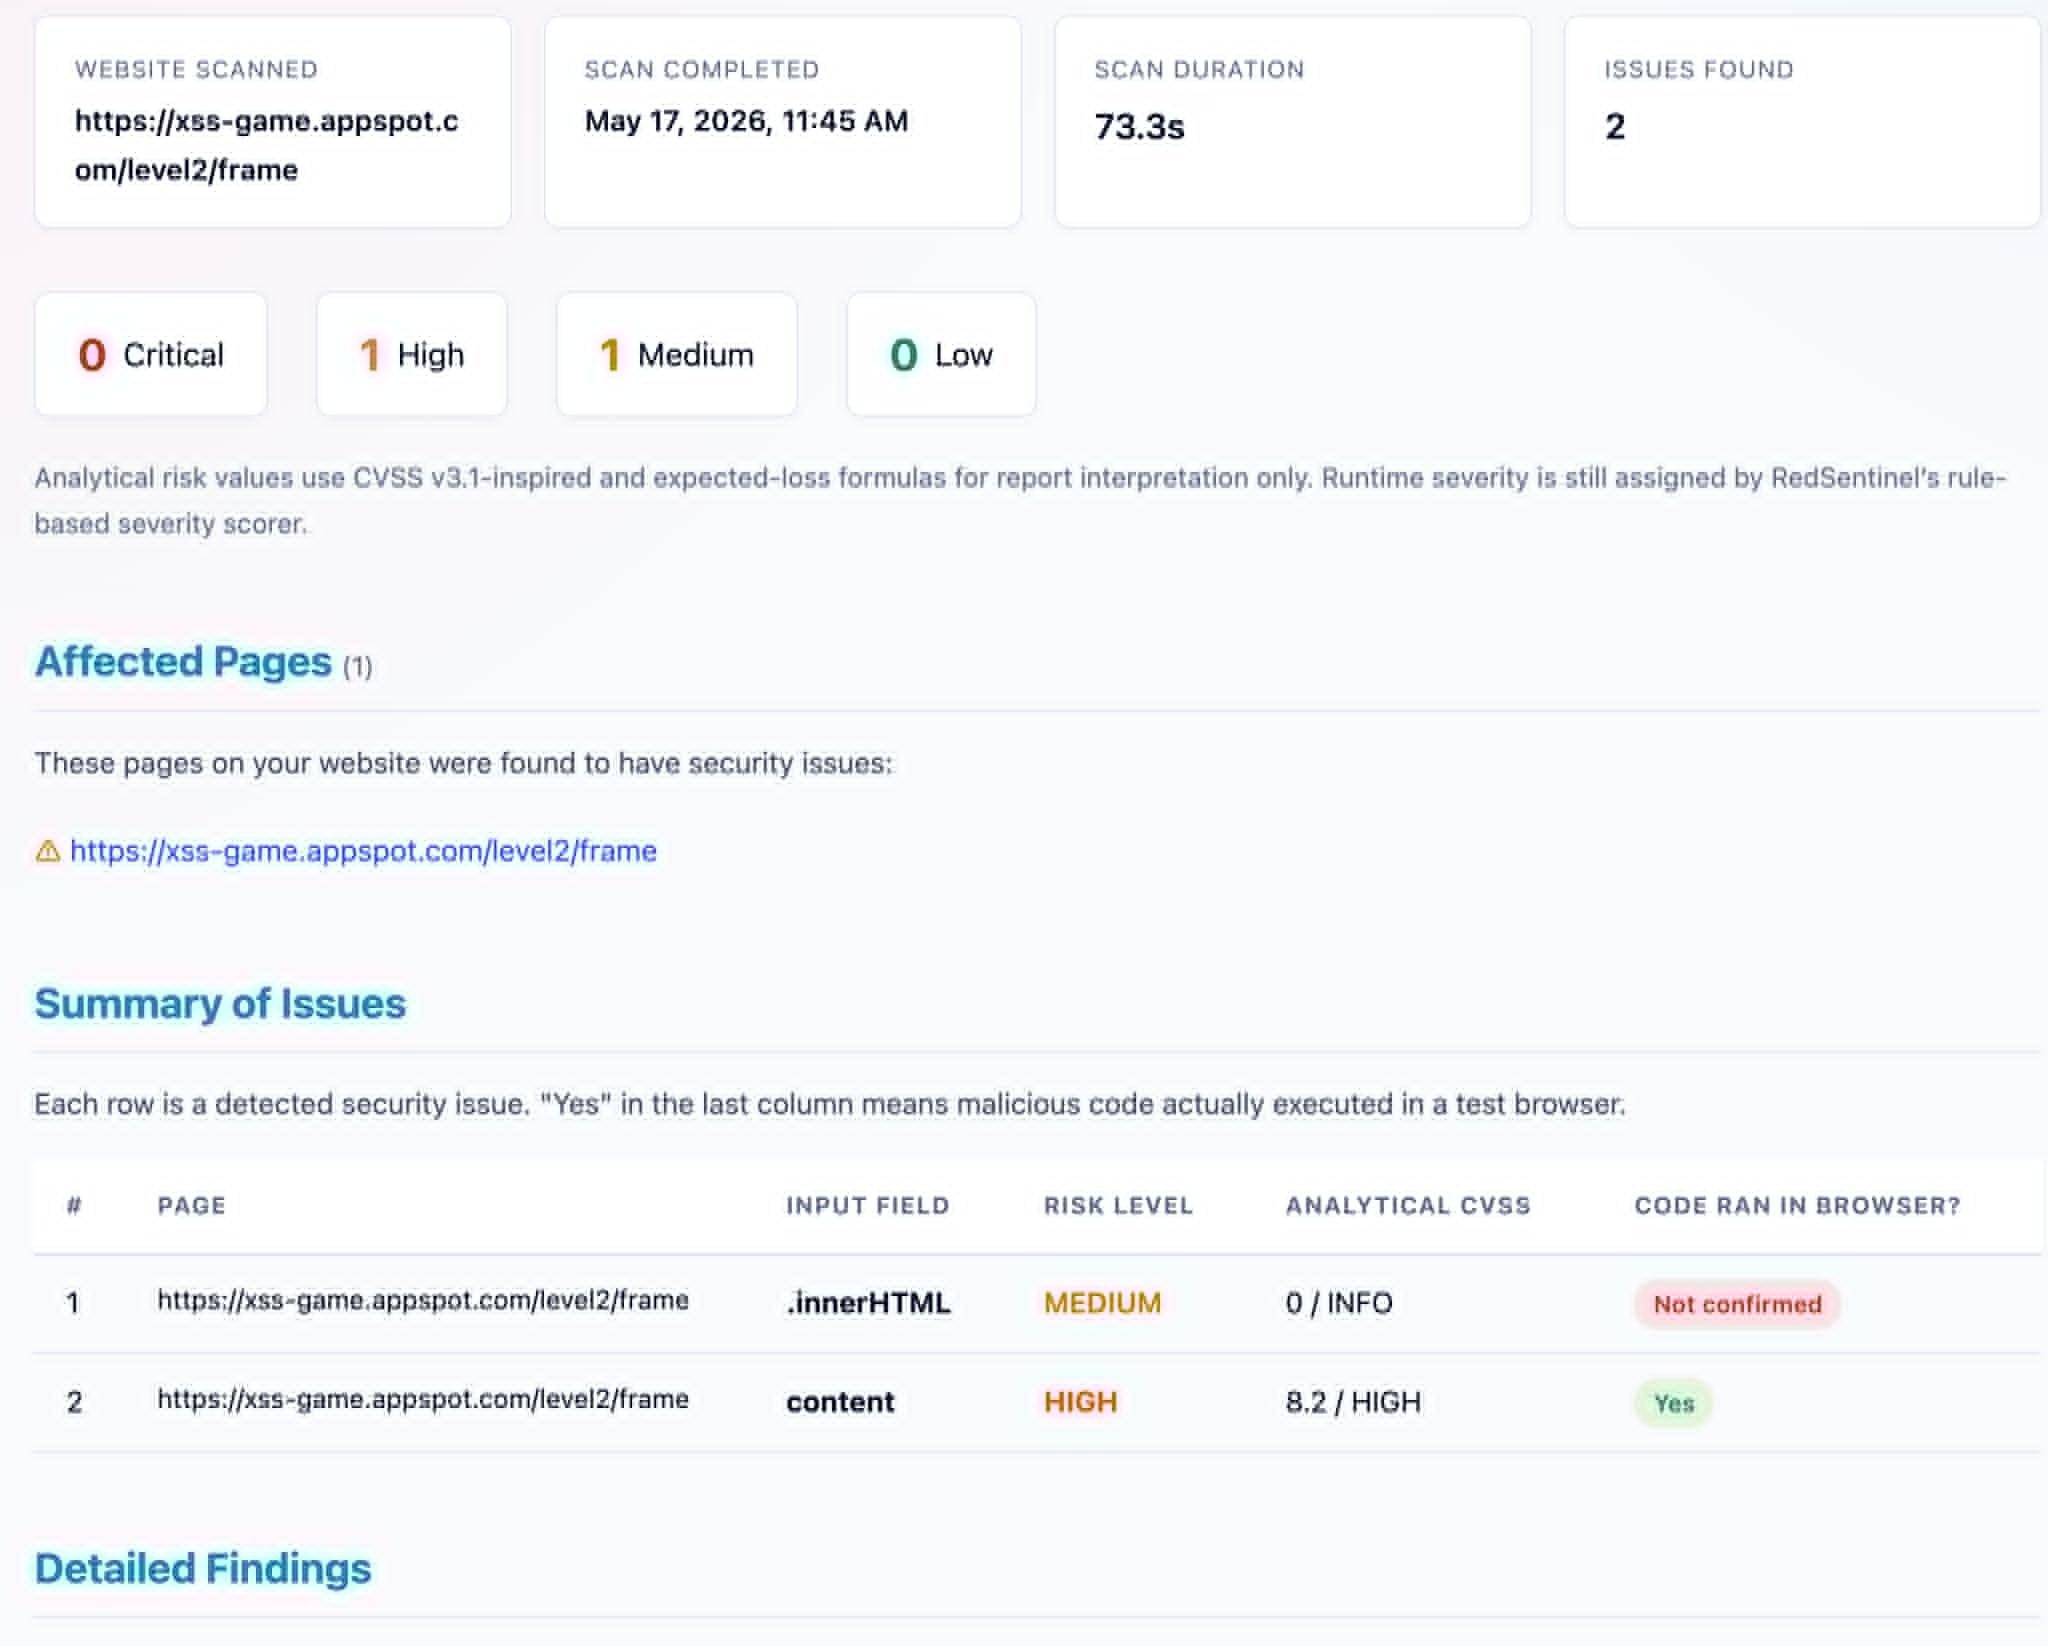
\includegraphics[width=1\linewidth]{figures/appendix/scanresult0.jpg}
    \caption{Scan summary report for \texttt{xss-game.appspot.com/level2/frame}.}
    \label{fig:appendixl0}
\end{figure}
\begin{figure}[H]
    \centering
    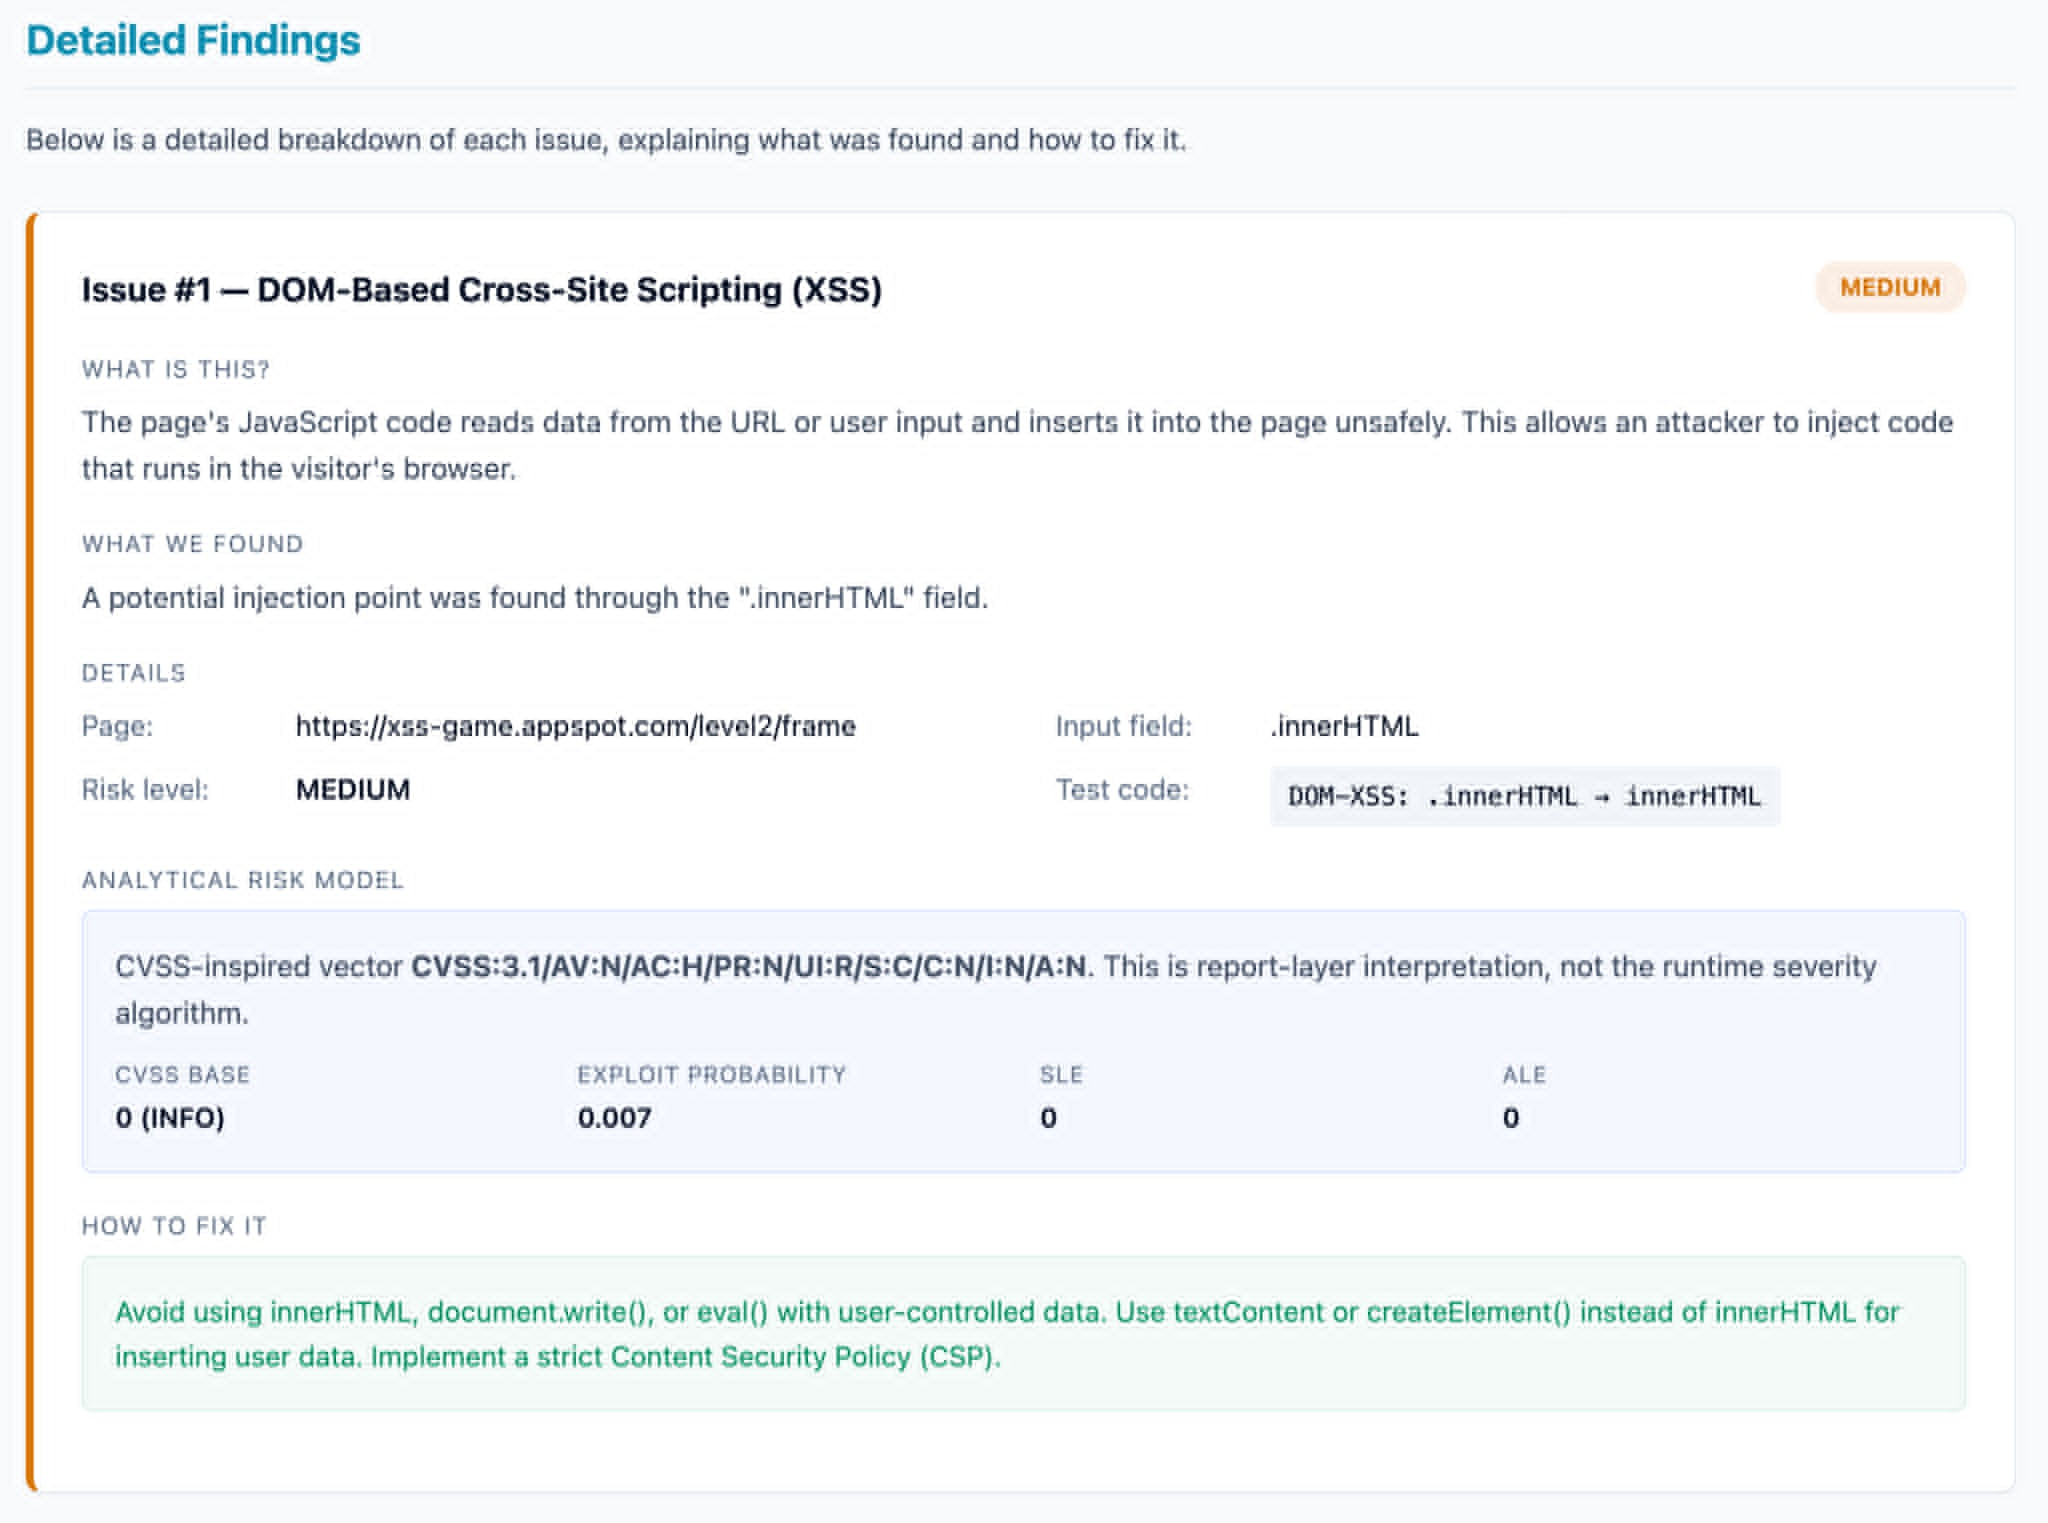
\includegraphics[width=0.9\linewidth]{figures/appendix/scanresult1.jpg}
    \caption{Issue \#1 --- DOM-Based Cross-Site Scripting (XSS) vulnerability report (severity: MEDIUM). A potential injection point was identified via the \texttt{.innerHTML} field at \texttt{xss-game.appspot.com/level2/frame}.}
    \label{fig:appendix_issue_high}
\end{figure}
\begin{figure}[H]
    \centering
    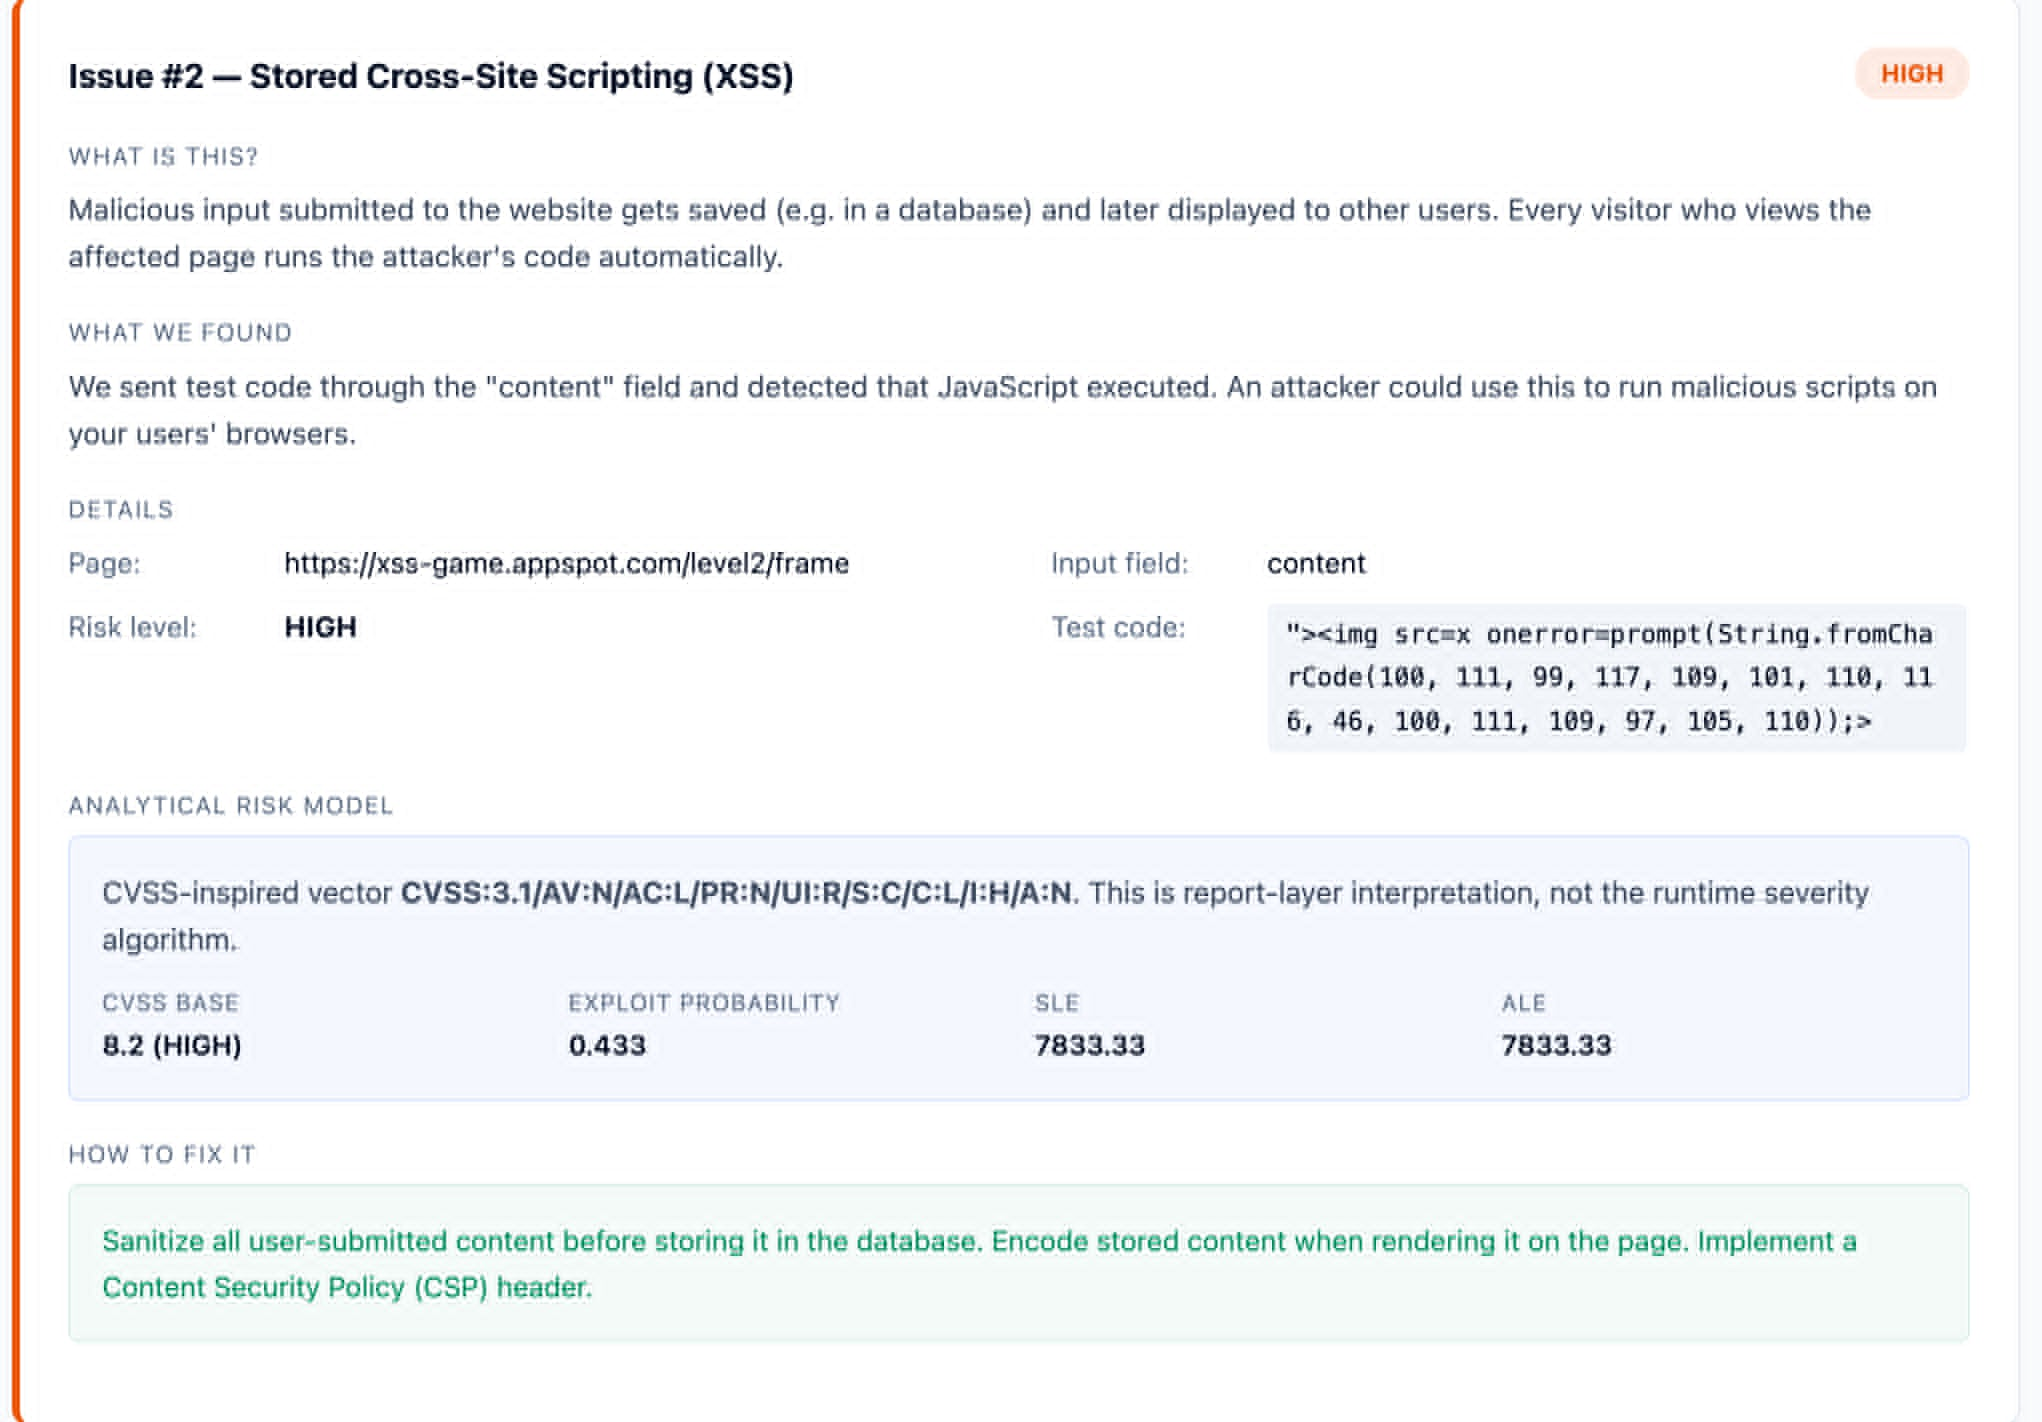
\includegraphics[width=0.9\linewidth]{figures/appendix/scanresult.jpg}
    \caption{Issue \#2 --- Stored Cross-Site Scripting (XSS) vulnerability report (severity: HIGH). The \texttt{content} input field at \texttt{xss-game.appspot.com/level2/frame} was found to execute injected JavaScript.}
    \label{fig:appendix_issue_critical}
\end{figure}
\clearpage
\renewcommand{\thefigure}{B.\arabic{figure}}
\renewcommand{\thetable}{B.\arabic{table}}
\setcounter{figure}{0}
\setcounter{table}{0}

\chapter*{Appendix B: RedSentinel Runtime Data Flow}
\addcontentsline{toc}{section}{Appendix B: RedSentinel Runtime Data Flow}

\begingroup
\small

\section*{B.1 Overview}

This appendix summarises the runtime data flow of RedSentinel from scan creation to final report generation. The purpose is to show the main data structures exchanged between the dashboard, core API, queue, Python microservices, target application, report engine, and training collector.

\begin{lstlisting}[style=appendixcode,caption={Overall scan pipeline}]
User Input
  -> Dashboard
  -> Core API
  -> BullMQ Queue
  -> Crawler
  -> Context Module
  -> Payload Generation Module
  -> Fuzzer Module
  -> Target Application
  -> Reflection / DOM / Browser Verification
  -> Severity and Risk Scoring
  -> Report Generation
  -> Runtime Training Data Collection
\end{lstlisting}

\section*{B.2 Dashboard Scan Request}

The scan begins when the user submits a target URL and scan options through the dashboard.

\begin{lstlisting}[style=appendixcode,caption={Dashboard to Core API request}]
POST http://localhost:4000/api/scans
Content-Type: application/json

{
  "url": "http://localhost:9090/reflected/body?q=test",
  "options": {
    "singlePage": true,
    "maxParams": 10,
    "verifyExecution": true,
    "maxPayloadsPerParam": 50,
    "timeout": 30000,
    "wafBypass": false
  }
}
\end{lstlisting}

\begin{lstlisting}[style=appendixcode,caption={Core API scan creation response}]
{
  "id": "62587fda-d7d2-4545-ad2b-321ab30c28a4",
  "url": "http://localhost:9090/reflected/body?q=test",
  "status": "PENDING",
  "progress": 0,
  "phase": "CRAWL",
  "createdAt": "2026-05-21T10:30:00.000Z"
}
\end{lstlisting}

\section*{B.3 Optional Authentication Data}

If the target requires authentication, the scan options may include cookie-based or login-based credentials.

\begin{lstlisting}[style=appendixcode,caption={Optional authentication options}]
{
  "auth": {
    "type": "cookie",
    "cookie": "session=abc123def456",
    "username": "admin",
    "password": "admin123"
  }
}
\end{lstlisting}

When authentication is not supplied, the scan continues as an unauthenticated scan.

\section*{B.4 WebSocket Progress Events}

The dashboard subscribes to scan events using the scan ID.

\begin{lstlisting}[style=appendixcode,caption={WebSocket subscription message}]
{
  "event": "subscribe",
  "data": {
    "scanId": "62587fda-d7d2-4545-ad2b-321ab30c28a4"
  }
}
\end{lstlisting}

Typical progress events are:

\begin{lstlisting}[style=appendixcode,caption={WebSocket scan event sequence}]
{"event":"scan.update","data":{"status":"CRAWLING","progress":5,"phase":"CRAWL"}}
{"event":"scan.update","data":{"status":"ANALYZING","progress":25,"phase":"CONTEXT"}}
{"event":"scan.update","data":{"status":"GENERATING","progress":50,"phase":"PAYLOAD_GEN"}}
{"event":"scan.update","data":{"status":"FUZZING","progress":75,"phase":"FUZZ"}}
{"event":"scan.vuln","data":{"param":"q","type":"reflected_xss","severity":"HIGH"}}
{"event":"scan.update","data":{"status":"REPORTING","progress":90,"phase":"REPORT"}}
{"event":"scan.done","data":{"status":"DONE","progress":100}}
\end{lstlisting}

\section*{B.5 Core Scan Record and Queue Job}

The core service stores the scan as a database record.

\begin{lstlisting}[style=appendixcode,caption={Simplified scan database record}]
{
  "id": "62587fda-d7d2-4545-ad2b-321ab30c28a4",
  "url": "http://localhost:9090/reflected/body?q=test",
  "status": "PENDING",
  "phase": "CRAWL",
  "progress": 0,
  "options": {
    "singlePage": true,
    "verifyExecution": true,
    "maxPayloadsPerParam": 50
  },
  "createdAt": "2026-05-21T10:30:00.000Z",
  "updatedAt": "2026-05-21T10:30:00.000Z",
  "completedAt": null,
  "error": null
}
\end{lstlisting}

A BullMQ job is then created for asynchronous processing.

\begin{lstlisting}[style=appendixcode,caption={BullMQ scan job payload}]
{
  "name": "scan",
  "jobId": "62587fda-d7d2-4545-ad2b-321ab30c28a4",
  "data": {
    "scanId": "62587fda-d7d2-4545-ad2b-321ab30c28a4"
  },
  "attempts": 3
}
\end{lstlisting}

\section*{B.6 Crawl Output}

The crawler converts the submitted URL into a list of testable endpoints and parameters.

\begin{lstlisting}[style=appendixcode,caption={Crawler output for single-page scan}]
[
  {
    "url": "http://localhost:9090/reflected/body",
    "method": "GET",
    "params": ["q"],
    "source": "url",
    "examples": {
      "q": "test"
    }
  }
]
\end{lstlisting}

For recursive scans, the same format is repeated for all discovered links, forms, and API endpoints.

\section*{B.7 Context Module Input and Output}

The crawler output is sent to the Context Module for reflection and context analysis.

\begin{lstlisting}[style=appendixcode,caption={Context Module input}]
{
  "endpoints": [
    {
      "url": "http://localhost:9090/reflected/body",
      "method": "GET",
      "params": ["q"],
      "examples": {
        "q": "test"
      }
    }
  ]
}
\end{lstlisting}

The Context Module injects a probe marker and records whether the marker is reflected.

\begin{lstlisting}[style=appendixcode,caption={Probe request format}]
GET http://localhost:9090/reflected/body?q=rs0xa1b2c3d4
\end{lstlisting}

\begin{lstlisting}[style=appendixcode,caption={Context Module output}]
{
  "endpoint": "http://localhost:9090/reflected/body?q=test",
  "params": [
    {
      "name": "q",
      "reflects": true,
      "context": "html_body",
      "context_confidence": 0.97,
      "reflection_position": "html_body",
      "probe_marker": "rs0xa1b2c3d4",
      "probe_method": "GET",
      "allowed_chars": ["<", ">", "\"", "'", "/", "\\", "(", ")", "{", "}", ";", "=", "`", "&", "|"]
    }
  ]
}
\end{lstlisting}

\section*{B.8 Payload Generation Input and Output}

The context result is sent to the Payload Generation Module.

\begin{lstlisting}[style=appendixcode,caption={Payload Generation Module input}]
POST http://localhost:5002/generate

{
  "endpoint_url": "http://localhost:9090/reflected/body",
  "context": "html_body",
  "params": {
    "q": {
      "reflects": true,
      "allowed_chars": ["<", ">", "\"", "'", "/", "\\", "(", ")", "{", "}", ";", "=", "`", "&", "|"]
    }
  },
  "max_payloads": 50,
  "waf_bypass": false
}
\end{lstlisting}

The module returns ranked, context-matched payloads.

\begin{lstlisting}[style=appendixcode,caption={Payload Generation Module output}]
{
  "payloads": [
    {
      "payload": "<img src=x onerror=alert(1)>",
      "target_param": "q",
      "confidence": 0.89,
      "technique": "original",
      "severity": "medium"
    },
    {
      "payload": "<svg onload=alert(1)>",
      "target_param": "q",
      "confidence": 0.87,
      "technique": "original",
      "severity": "medium"
    },
    {
      "payload": "<script>alert(1)</script>",
      "target_param": "q",
      "confidence": 0.85,
      "technique": "original",
      "severity": "medium"
    }
  ]
}
\end{lstlisting}

\section*{B.9 Fuzzer Module Input}

The selected payloads are sent to the Fuzzer Module.

\begin{lstlisting}[style=appendixcode,caption={Fuzzer Module input}]
POST http://localhost:5003/fuzz

{
  "url": "http://localhost:9090/reflected/body",
  "payloads": [
    {
      "payload": "<img src=x onerror=alert(1)>",
      "target_param": "q",
      "confidence": 0.89,
      "technique": "original",
      "severity": "medium"
    }
  ],
  "verify_execution": true,
  "timeout": 60000,
  "stored_mode": false
}
\end{lstlisting}

\section*{B.10 HTTP Request and Response Data}

The fuzzer injects each payload into the target parameter.

\begin{lstlisting}[style=appendixcode,caption={Fuzzer HTTP request}]
GET /reflected/body?q=%3Cimg%20src%3Dx%20onerror%3Dalert(1)%3E HTTP/1.1
Host: localhost:9090
User-Agent: Mozilla/5.0 (compatible; RedSentinel/1.0)
Accept: text/html
\end{lstlisting}

\begin{lstlisting}[style=appendixcode,caption={Target HTTP response}]
HTTP/1.1 200 OK
Content-Type: text/html; charset=utf-8

<html>
<body>
  <p>You entered: <b><img src=x onerror=alert(1)></b></p>
</body>
</html>
\end{lstlisting}

The raw fuzzer result is stored in the following format.

\begin{lstlisting}[style=appendixcode,caption={Raw fuzzer result format}]
{
  "payload": "<img src=x onerror=alert(1)>",
  "target_param": "q",
  "url_sent": "http://localhost:9090/reflected/body?q=%3Cimg%20src%3Dx%20onerror%3Dalert(1)%3E",
  "status_code": 200,
  "response_headers": {
    "Content-Type": "text/html; charset=utf-8"
  },
  "response_snippet": "...<b><img src=x onerror=alert(1)></b>...",
  "reflected": false,
  "executed": false,
  "vuln": false,
  "evidence": {}
}
\end{lstlisting}

\section*{B.11 Reflection Check Output}

The reflection checker updates the result after comparing the payload with the HTTP response.

\begin{lstlisting}[style=appendixcode,caption={Reflection check output}]
{
  "payload": "<img src=x onerror=alert(1)>",
  "reflected": true,
  "exact_match": true,
  "reflection_position": "html_body",
  "reflection_snippet": "...<b><img src=x onerror=alert(1)></b>..."
}
\end{lstlisting}

\section*{B.12 DOM XSS Scan Output}

For DOM-based targets, the scanner records source-to-sink evidence.

\begin{lstlisting}[style=appendixcode,caption={DOM XSS scan result format}]
{
  "dom_vuln": true,
  "source": "URLSearchParams.get",
  "sink": "innerHTML",
  "line": 6,
  "snippet": "document.getElementById('output').innerHTML = data;"
}
\end{lstlisting}

\section*{B.13 Browser Verification Output}

If browser verification is enabled, reflected payloads are opened in a headless browser.

\begin{lstlisting}[style=appendixcode,caption={Browser verification output}]
{
  "payload": "<img src=x onerror=alert(1)>",
  "executed": true,
  "dialog_triggered": true,
  "dialog_type": "alert",
  "dialog_text": "1",
  "console_errors": [],
  "confirmed": true
}
\end{lstlisting}

A non-executing reflected payload is stored as:

\begin{lstlisting}[style=appendixcode,caption={Negative browser verification output}]
{
  "payload": "<script>alert(1)</script>",
  "reflected": true,
  "executed": false,
  "dialog_triggered": false,
  "confirmed": false
}
\end{lstlisting}

\section*{B.14 Final Fuzzer Result}

The Fuzzer Module returns one result object per payload.

\begin{lstlisting}[style=appendixcode,caption={Final fuzzer result format}]
{
  "results": [
    {
      "payload": "<img src=x onerror=alert(1)>",
      "target_param": "q",
      "vuln": true,
      "type": "reflected_xss",
      "reflected": true,
      "exact_match": true,
      "executed": true,
      "dialog_triggered": true,
      "reflection_position": "html_body",
      "technique": "original",
      "severity": "high",
      "evidence": {
        "responseCode": 200,
        "reflectionPosition": "html_body",
        "browserAlertTriggered": true,
        "exactMatch": true,
        "response_snippet": "...<b><img src=x onerror=alert(1)></b>..."
      },
      "context_classification": {
        "param": "q",
        "context": "html_body",
        "method": "GET",
        "confidence": 0.97
      }
    }
  ]
}
\end{lstlisting}

\section*{B.15 Severity and Risk Output}

The core service calculates severity for each confirmed vulnerability.

\begin{lstlisting}[style=appendixcode,caption={Severity score format}]
{
  "severityScore": 80,
  "severity": "HIGH",
  "severityBreakdown": {
    "execution": 40,
    "shareability": 30,
    "sinkDanger": 10,
    "payload": 10
  }
}
\end{lstlisting}

The scan-level risk result is stored as:

\begin{lstlisting}[style=appendixcode,caption={Risk analysis format}]
{
  "riskScore": 85,
  "riskLevel": "CRITICAL",
  "topVulnType": "reflected_xss",
  "exploitableWithoutAuth": true,
  "browserConfirmedCount": 18,
  "totalVulnCount": 18
}
\end{lstlisting}

\section*{B.16 Final Report Data Format}

The report engine generates JSON, HTML, and PDF reports. The JSON report follows this structure.

\begin{lstlisting}[style=appendixcode,caption={Final report format}]
{
  "scanId": "62587fda-d7d2-4545-ad2b-321ab30c28a4",
  "url": "http://localhost:9090/reflected/body?q=test",
  "status": "DONE",
  "summary": {
    "totalPayloads": 50,
    "reflected": 42,
    "executed": 18,
    "confirmedVulns": 18,
    "severityBreakdown": {
      "CRITICAL": 3,
      "HIGH": 8,
      "MEDIUM": 5,
      "LOW": 2,
      "INFO": 0
    }
  },
  "vulns": [
    {
      "id": "vuln-001",
      "param": "q",
      "payload": "<img src=x onerror=alert(1)>",
      "type": "reflected_xss",
      "severity": "HIGH",
      "url": "http://localhost:9090/reflected/body?q=%3Cimg%20src%3Dx%20onerror%3Dalert(1)%3E",
      "reflected": true,
      "executed": true,
      "evidence": {
        "responseCode": 200,
        "reflectionPosition": "html_body",
        "browserAlertTriggered": true,
        "exactMatch": true,
        "severityScore": 80
      }
    }
  ],
  "riskAnalysis": {
    "riskScore": 85,
    "riskLevel": "CRITICAL"
  },
  "metadata": {
    "target": "http://localhost:9090",
    "targetName": "exploitable",
    "scanDuration": "60.2s",
    "fuzzerVersion": "1.0.0"
  }
}
\end{lstlisting}

\section*{B.17 Runtime Training Sample Format}

After fuzzing, useful runtime results are appended to the ranker-training JSONL file.

\begin{lstlisting}[style=appendixcode,caption={Runtime training sample format}]
{
  "timestamp": "2026-05-21T12:00:00.123456",
  "url": "http://localhost:9090/reflected/body",
  "payload_text": "<img src=x onerror=alert(1)>",
  "target_param": "q",
  "context": "html_body",
  "waf": "none",
  "technique": "original",
  "severity": "medium",
  "allowed_chars": ["<", ">", "\"", "'", "/", "\\", "(", ")", "{", "}", ";", "=", "`", "&", "|"],
  "response_snippet": "...<b><img src=x onerror=alert(1)></b>...",
  "sink_name": null,
  "source_name": null,
  "dataflow": null,
  "executed": true,
  "dialog_triggered": true,
  "reflected": true,
  "exact_match": true,
  "reflection_position": "html_body",
  "success": true
}
\end{lstlisting}

\section*{B.18 Evaluation Result Format}

The evaluation pipeline compares expected and detected vulnerabilities.

\begin{lstlisting}[style=appendixcode,caption={Evaluation metric format}]
{
  "tp": 14,
  "fn": 1,
  "tn": 1,
  "fp": 0,
  "precision": 1.0,
  "recall": 0.933,
  "f1": 0.965
}
\end{lstlisting}

Evaluation archives follow this structure.

\begin{lstlisting}[style=appendixcode,caption={Evaluation archive structure}]
eval/archive/2026-05-21_10-30-00/
|-- _meta.json
|-- manifest_frozen.json
|-- results/
|   |-- reflected-body.json
|   |-- reflected-attribute.json
|   |-- dom-innerhtml.json
|   |-- raw_responses/
|       |-- reflected-body.json
|-- summary.json
|-- portswigger.json
\end{lstlisting}

\section*{B.19 Stored XSS Data Flow Format}

Stored XSS follows the same pipeline but uses a submit-and-poll structure.

\begin{lstlisting}[style=appendixcode,caption={Stored XSS crawler output}]
[
  {
    "url": "http://localhost:9090/stored/comments",
    "params": ["name", "body"],
    "method": "POST",
    "form": true,
    "stored_endpoint": true
  },
  {
    "url": "http://localhost:9090/stored/comments",
    "params": [],
    "method": "GET",
    "renders_stored_data": true
  }
]
\end{lstlisting}

\begin{lstlisting}[style=appendixcode,caption={Stored XSS final result format}]
{
  "scanId": "scan-002",
  "url": "http://localhost:9090/stored/comments",
  "status": "DONE",
  "summary": {
    "totalPayloads": 3,
    "confirmedVulns": 1,
    "severityBreakdown": {
      "HIGH": 1
    }
  },
  "vulns": [
    {
      "param": "body",
      "payload": "<img src=x onerror=alert(1)>",
      "type": "stored_xss",
      "severity": "HIGH",
      "executed": true,
      "stored": true,
      "evidence": {
        "submitMethod": "POST",
        "pollUrl": "http://localhost:9090/stored/comments",
        "browserAlertTriggered": true
      }
    }
  ]
}
\end{lstlisting}

\section*{B.20 Summary}

The runtime flow shows that RedSentinel records each major object passed through the system: user scan options, scan database record, queue job, crawler output, context classification result, generated payloads, fuzzing request, HTTP response evidence, reflection result, DOM result, browser-verification result, severity score, risk score, final report, and runtime training sample.

\endgroup